%************************************************
\section{Black-Box Analysis}\label{ch:Blackbox}
%************************************************
In this section, we introduce black-box analysis and how we use it to analyze configurable software systems. 
In \autoref{ch:bb-general-concept}, we explain the general concepts of a black-box and black-box analysis. 
Afterwards, we highlight the challenges we encounter when using a black-box analysis.
After using the black-box analysis, we use the obtained data, to build a performance-influence model using multiple linear regression in \autoref{ch:linear-regression}.

\begin{figure}[h]
    \centering
    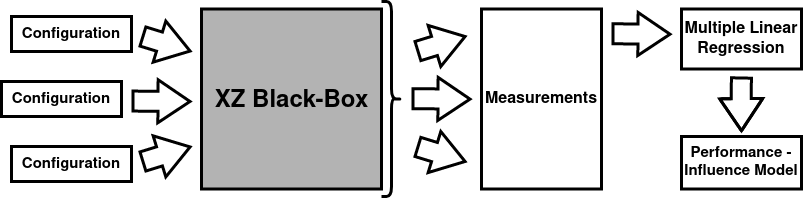
\includegraphics[scale=0.53]{gfx/BlackBox2_0.png}
    \caption{Process of using a black-box analysis to build a {\perfInfluenceModel} for \textit{XZ}.}
    \label{fig:BBxz}
\end{figure}

%Example of Chapter pipeline
In \autoref{fig:BBxz}, we use a black-box analysis for \textit{XZ} to build a \perfInfluenceModel.
We start by focusing on finding the features that we are interested in. 
Then we build ourselves multiple configurations that hold different interactions between these features.
Afterwards, we run \textit{XZ} as a black-box on each configuration; during the execution, we analyze the system by measuring different non-functional properties.
In our case, we are interested in the performance of each feature. 
We repeat this process for each configuration during the black-box analysis and collect the measurements.
Next, we use these measurements together with multiple linear regression to build a \perfInfluenceModel.

\subsection{General Concepts}\label{ch:bb-general-concept}

%Introduction why now black-box
We have introduced {\perfInfluenceModel} to represent each feature and feature interaction's influences. 
In this section, we expand on this topic and introduce the \emph{black-box analysis} a method to collect data to build \perfInfluenceModel.

%What is a black-box and what is the analysis
A black-box of a configurable system is conceptually simple, we execute a given system with a configuration, and after finishing, we receive an output. 
However, the critical part is that we are unaware of how the black-box produces the output. 
Since we cannot see inside the system, we need an approach that does not require this. 
Therefore, in a black-box analysis, we solve this issue by observing the machine on which the system is executed and 
collect measurements for the non-functional property we are interested in.

%\subsection{Black-Box Analysis}\label{ch:Black-Box-Analysis}
%Intro in section, combinatorial explosion
However, before we start analyzing the system, we first have to select the features we are interested in, since for most configurable systems it is 
not feasible to use the whole configuration space due to its size. This issue is called \emph{combinatorial explosion} in \autoref{section:combinatorial-explosion}
we explain how we deal with this problem.

%The analysis
After deciding which features are of interest to us, we can now turn to the question 
of how we analyze the system and collect the data we need to build a {\perfInfluenceModel}.

As shown in \autoref{fig:BBxz}, we cannot analyze how the system produces the output; 
therefore, we are limited to the non-functional properties we can observe from the outside. For this reason, 
we execute the system with each configuration and measure the property we are interested in, such as energy consumption, memory usage, 
and computational resources used.  

\subsubsection{Challenges}\label{section:combinatorial-explosion}
%Defining combinatorial explosion
One of the larger problems we face when using black-box analysis is the issue of combinatorial explosion, 
which refers to the effect that when features increase linearly, the number of possible configuration
increase exponentially~\cite{Combinatorial-explosion}.

%Explaining exponential groth more in detail
Suppose we have a configurable system where each feature is a binary option.
We also define that in this system, each feature is entirely independent of another
(i.e., the system has no constraints, and selecting or deselecting one feature has no effect on other features).
The number of unique configurations this system can produce is $2^n$, where $2$ refers to the type of feature options allowed,
binary in our case, and $n$ denotes the number of features. 

%Why it is a problem, Example
The problem, is that all these different features can interact with each other in different ways, and for very small systems
we can certainly brute force our way by benchmarking all possible configuration, however this does not scale.
So, the brute force-method is not feasible for larger systems. 

%Example    
To illustrate the problem, the Linux kernel contains 10`000 different features~\cite{Linux-Kernel}, thus there are $2^{10000}$
possible configurations.
It is estimated that the universe
contains about $10^{79}$ atoms, which is still less than the number of unique configurations a system with 263 features produces.
Such a system is already impossible to analyze using brute force, let alone the Linux kernel.

%How wo overcome it
Hence, we cannot fully explore the entire configuration space and must select a subset representing the system with high accuracy. 
One way to solve this issue is to select different configurations from the configuration space using a sampling strategy.
Whereas in this work, we take advantage of the findings of Xu et al.~\cite{TooManyKnobs}, 
where they have shown that not all features are equally important and that up to 54,1\% of features are rarely set by users. 
We use this information together with our domain knowledge to extract the most important features we are interested in.


\subsection{Multiple Linear Regression} \label{ch:linear-regression}
%Section overview
After we used the black-box analysis to collect measurements of the all the configuration are interested in, 
we use them to build our {\perfInfluenceModel} of the system. 
This section explains the reasoning behind using \emph{multiple linear regression}. 
Afterwards, in \autoref{ch:OLS}, we explain \emph{ordinary least squares}, an estimator to calculate the coefficient of each term inside the \perfInfluenceModel. 
When using \emph{ordinary least squares} as an estimator, we have to handle \emph{multicollinear features}. 
We explain why multicollinear features are a problem in \autoref{ColinearF} and how to reduce the influence of them by using
 \emph{Variance Inflation Factor} in \autoref{ch:vif}.

%Why Multiple limear regression
When building a {\perfInfluenceModel} from our black-box data we have would like our model to be interpretable. While multiple 
methods to predict performance have been introduced, such as neural networks, they lack the interpretability of the model, which on contrary
\emph{multiple linear regression} provides.

To illustrate why interpretability is important lets inspect the following \perfInfluenceModel:

\begin{align*}
    \Pi_1 &= -1000 + 1001 \cdot \textit{Feature\_A} + 1002 \cdot \textit{feature\_B} - 1000 \cdot \textit{Feature\_A} \cdot \textit{feature\_B} \\
    \Pi_2 &= 0 + 1 \cdot \textit{Feature\_A} + 2 \cdot \textit{feature\_B} + 0 \cdot \textit{Feature\_A} \cdot \textit{feature\_B}
\end{align*}

%Example why we need interpretability
Under the condition that either \textit{Feature\_A} or \textit{Feature\_B} needs to be selected, 
$\Pi_1$ and $\Pi_2$ predict for any configuration the same amount of time, however, 
if we take a close look at how $\Pi_1$ assigns the influence of each feature, we can see that this is not interpretable. 
Here $\Pi_1$ assigns to the \textit{Base} feature an influence of -1000 thousand, 
which does not make sense since the time spent in the \textit{Base} feature can not be negative. 
This also leads to $\Pi_1$ assigning unrealistic amounts of time to features or feature interactions. 

To build the {\perfInfluenceModel} using the measurements from the black-box analysis we use 
 the following formula for multiple linear regression for matrices ~\cite{Linear-Regression-Performance}:

\begin{align}\label{formula:linReg}
    Y &= \beta_0 + \beta_1 x_1 + \beta_2 x_2 ... \beta_n x_n + \epsilon   \\
    Y &= X \beta + \epsilon \nonumber\\ \nonumber \\ \nonumber
    Y &= \textit{Dependent variable}\\ \nonumber
    X &= \textit{Independent variable}\\ \nonumber
    \beta &= \textit{Regression coefficient}\\ \nonumber
    \epsilon &= \textit{Error} \nonumber
\end{align}

%For what linear reg is used
In our case, $Y$ is a vector with \textit{n}  elements containing the output of our black-box model,
i.e., the measurements for each configuration in our set of configurations $\mathcal{C}$. 

%Exlaining collums of matrix and how they map to our config
Our independent variable $X$ is an $n \times m$ matrix, where $n$ is the number of configurations used, 
and $m$ is the number of features and feature interactions across all configurations. 
To accommodate feature interactions in this linear model, we add a term for each interaction we want to include. 
For example, if we consider the interaction between features $x_i$ and $x_j$ we add the term $\beta_k x_i x_j$. 

%Explaining coecfficient map to feature
We are interested in the values of the coefficients $\beta$, since they quantify the influence of each feature or feature interaction on the whole system. 
In addition, $\beta_0$ denotes the intercept, representing the influence of the base code, 
meaning the part of the code executed regardless of the chosen configuration.

%Splitting of feature interactions
The value of each feature in the matrix is $1$ if the feature is selected or $0$ if it is not selected.  If we have numerical features with $l$ different options, 
we split these features into $l$ binary features and encode them as an alternative group in our feature model.

%Error
All our measurements have a possible error represented by $\epsilon$~\cite{Linear-Regression}.

\subsubsection{Ordinary Least Squares}\label{ch:OLS}
%Why we need ols
Now that we have seen the general formula of multiple linear regression and know what the different components stand for, we still need to figure out 
how to calculate the regression coefficient $\beta$ and the values that tell us the influence of each feature. 

%Why OLS works in detail
For this purpose, we use the ordinary least squares estimator, which is optimal for the class of linear unbiased estimators, 
but is unreliable when the independent variables $X$ contains a high degree of multicollinearity.
The problem of multicollinearity is later explained in detail in \autoref{ColinearF}.
Ordinary least squares minimizes the sum of the squared residuals, where the residual is the difference between
the predicted value of the estimator and the actual value~\cite{Linear-Regression}.


\begin{figure}[H]
    \centering
    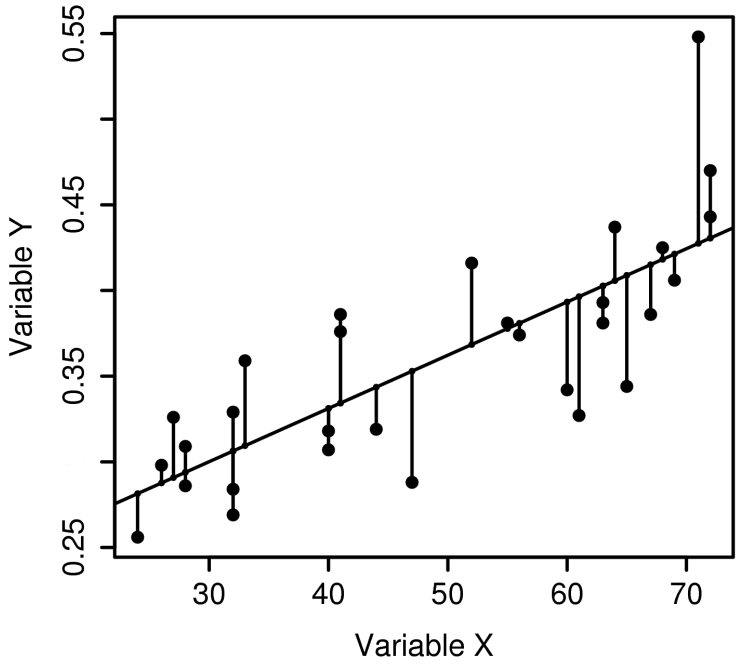
\includegraphics[scale=0.3]{gfx/OLS.png}
    \caption[Ordinary Least Squares regression model residuals]
    {Ordinary Least Squares regression model residuals
    \footnotemark .}
    \label{fig:OLS}
\end{figure}
\footnotetext{Visited at 06.03.2023, \url{https://datajobs.com/data-science-repo/OLS-Regression-[GD-Hutcheson].pdf}}

%example illustration
We see an illustration of an ordinary least squares estimator for a linear regression model in \autoref{fig:OLS}. In which we have only one variable 
X and the corresponding measurements Y, allowing us to compute the single regressor for this linear regression model.

To compute the regression coefficients using ordinary least squares, the following formula is used~\cite{Linear-Regression}:

\begin{align}
    \hat{\beta} &=  (\textit{X}^{\top } \textit{X} )^{-1}\textit{X}^{\top} Y \\ \nonumber \\\nonumber
    \hat{\beta} &= \textit{Ordinary Least Squares Estimator}\\\nonumber
    \top &= \textit{Matrix Transposed}\nonumber
\end{align}\label{equ:ols}

For us $\hat{\beta}$ contains all the regression coefficient we are interested in, i.e. the predicted time spent for each feature or feature interaction.

We proceed with an example of using ordinary least squares to build a {\perfInfluenceModel}. 
We select some configurations and use the black-box analysis to measure the time spend using these configurations. 
The results are in \autoref{table:performanceExample-sample}.

\begin{table}[H]
    \centering
    \begin{tabular}{rrrrrrrr}
    \toprule
    Base & A & B & C & A $\land$ B & A $\land$ C &  & \textit{measured} \\ \midrule
    1    & 0 & 0 & 0 & 0           & 0           &  &  $\mathbf{1}$   \\
    1    & 1 & 0 & 0 & 0           & 0           &  &  $\mathbf{2}$   \\
    1    & 0 & 1 & 0 & 0           & 0           &  &   $\mathbf{3}$  \\  
    1    & 0 & 0 & 1 & 0           & 0           &  &   $\mathbf{2}$  \\  
    1    & 1 & 1 & 0 & 1           & 0           &  &   $\mathbf{6}$   \\
    1    & 1 & 0 & 1 & 0           & 1           &  &   $\mathbf{3}$  \\  
    1    & 0 & 1 & 1 & 0           & 0           &  &   $\mathbf{4}$  \\  
    1    & 1 & 1 & 1 & 1           & 1           &  &   $\mathbf{7}$  \\ \bottomrule
    \end{tabular}  
    \caption{Configuration samples of \autoref{lst:performanceExample}, 
    where \textit{measured} is the time we measure using the selected features in that row.}\label{table:performanceExample-sample}
\end{table}

Using the configuration samples from \autoref{tab:alternative} we can now determine $\textit{X}$ and $\textit{Y}$:

\begin{equation}\label{equ:exampleIndependentDependent}
    \textit{X} = 
    \begin{bmatrix} 
        1 & 0 & 0 & 0 & 0 & 0 \\
        1 & 1 & 0 & 0 & 0 & 0 \\
        1 & 0 & 1 & 0 & 0 & 0 \\
        1 & 0 & 0 & 1 & 0 & 0 \\
        1 & 1 & 1 & 0 & 1 & 0 \\
        1 & 1 & 0 & 1 & 0 & 1 \\
        1 & 0 & 1 & 1 & 0 & 0 \\
        1 & 1 & 1 & 1 & 1 & 1 
      \end{bmatrix}
      ,
      \textit{Y} =
      \begin{bmatrix}
        1 \\
        2 \\
        3 \\
        2 \\
        6 \\
        3 \\
        4 \\
        7 
      \end{bmatrix}
\end{equation}


Using the ordinary least squares \hyperref[equ:ols]{Equation \ref*{equ:ols}}  we obtain the following results:

\begin{equation}
    \hat{\beta} = 1 + 
    \begin{bmatrix}
        0,00 \\
        1,00 \\
        2,00 \\
        1,00 \\
        2,00 \\
        0,00
    \end{bmatrix}
\end{equation}

All values have been rounded to 2 decimal places. We can see that all values have been assigned correctly.

In this example, we choose the configurations we want to analyze and measure the time spent for each configuration using the black-box analysis. 
We collect the results in \autoref{table:performanceExample-sample}. 
Then as our independent variable \textit{Y} we use the time \textit{measured} for each configuration 
and for \textit{X} we use each feature or feature interaction we included in the configurations. 
Afterwards, we use the ordinary least squares formula of \autoref{equ:ols} with \textit{X} and \textit{Y} to calculate the regression coefficients $\hat{\beta}$. 
Now we can use the values to create the \perfInfluenceModel:

\begin{equation}\label{equ:performanceExamplePIMBlackBox}
    \Pi = 1 + 1 \cdot c(A) + 2 \cdot c(B) + 1 \cdot c(C) + 2 \cdot c(A) \cdot B + 0 \cdot c(A) \cdot c(C)
\end{equation}

\subsubsection{Multicollinear Features}\label{ColinearF}
%Connection/Explantion why multicolinearty is bad
We already mentioned that ordinary least squares is optimal as long as our configurations do not contain multicollinearity. The reason for that
is in presence of multicollinearity the variance of the estimator inflates, which in result hurts the interpretability of the model.
We call features multicollinear when there exist a near linear dependency between these features, meaning we can nearly represent one feature as a combination
of different features and the feature does only provide a small amount of new information to the system~\cite{Linear-Regression}. If a feature does not provide
any new information to the system, then we speak of perfect multicollinearity. 
As an example take a look at a {\perfInfluenceModel} for some the monthly expenses of a student, where \textit{take\_out} is included in the 
cost of \textit{food}:

\begin{equation*}
    monthly\_expenses = \textit{food} + \textit{take\_out}
\end{equation*}

%Explanation and example for perfect multicolinearity
Now this shows multicollinearity between the features \textit{food} and \textit{take\_out}, since \textit{take\_out} is already present in the cost of \textit{food},
furthermore it is a case of perfect multicollinearity, since the feature does not provide any new information.

One way multicollinearity is introduced into a system is by using alternative groups, since the selection of a feature in the
alternative group can be expressed by the combination of all other feature.~\cite{Multicollinearity}

\begin{table}[H]
    \centering
    \begin{tabular}{rrrrrr}
    \toprule
    Base & A & B & C &  & $\bm{\Pi(*)}$ \\ \midrule
    1 & 1 & 0 & 0 &  & $\mathbf{5}$  \\
    1 & 0 & 1 & 0 &  & $\mathbf{10}$  \\  
    1 & 0 & 0 & 1 &  & $\mathbf{15}$  \\\bottomrule
    \end{tabular}  
    \caption{Configuration example illustrating multicollinearity in an alternative group,
    where $\bm{\Pi(*)}$ is the predicted time for the selected feature inside the row.}\label{tab:alternative}
\end{table}

%Example alternative group
Now consider the example presented in \autoref{tab:alternative}, 
where we see a configuration example that contains multicollinear features \textit{A}, \textit{B}, and \textit{C} due to an alternative group.
The example contains a mandatory \textit{Base} feature and 3 features that are in an alternative to each other.
Now we can always model the presence of a feature in an alternative group due to the absence of other feature, here for feature \textit{C} to be selected, 
\textit{B} and \textit{A} needs to be deselected. This results in the following 3 {\perfInfluenceModel}s:


\begin{align*}
    \Pi_0(c) &= 0 + 5 \cdot c(A) + 10\cdot c(B) + 20\cdot c(C) \\
    \Pi_1(c) &= 5 + 10 \cdot c(A) + 5\cdot c(B) + 20\cdot c(C) \\
    \Pi_2(c) &= 8 + 20 \cdot c(A) + 10\cdot c(B) + 7\cdot c(C) \\
\end{align*}

This leads to multiple performance-influcence models that are accurate with respect to the individual measurement, 
but make completely different statements when compared.

\begin{table}[h]
    \centering
    \begin{tabular}{rrrrrrr}
    \hline
    $\Pi$ & Base & A & B & C   & &  $\bm{\Pi(\{Base\})}$   \\ \hline
    $\Pi_0$ & 0 & 5  & 10 & 20 & &  $\mathbf{0}$         \\
    $\Pi_1$ & 5 & 10 & 5  & 20 & &  $\mathbf{5}$         \\  
    $\Pi_2$ & 8 & 20 & 10 & 7  & &  $\mathbf{8}$        \\\hline
    \end{tabular}
    \caption{Performance predictions of \autoref{tab:alternative}}\label{tab:Performance-predictions}
\end{table}

The examples illustrated how multicollinearity is introduced when we use alternative groups. 
Therefore, when choosing the configuration space, this needs to be considered. 

%Explain multicollinearity 
Another way multicollinearity is introduced into the system is to have features that are mandatory or connected by a condition. 
If we have features that are mandatory, we cannot distinguish these features with our black-box analysis because they are always selected
together, and we cannot determine the extent to which each feature influences the system~\cite{Multicollinearity}.

%Multicolinearity with mandatory feature explaining examples before
In \autoref{tab:Performance-predictions}, we see the predictions each of the 3 {\perfInfluenceModel}s make for the configurations $\{Base\}$. 
Now $\Pi_0$, $\Pi_1$, and $\Pi_2$, assign completely different values to the \textit{Base} feature, which makes it impossible for, the user,
to infer the correct value. The reason is that both \textit{Base} and a feature of the alternative group are mandatory. 
Therefore, we cannot measure one without the presence of the other. 
Hence, the values of \textit{Base} or the alternative group feature can be set in any ratio as long as the sum of the two values equals the measured time.

In this section, we learned about multicollinearity and how alternative groups and mandatory features introduce multicollinearity into a system. 
When we decide which features to use in our configuration set, we use our domain knowledge of the system to reduce multicollinear features to a minimum.
To measure the degree of multicolinearity inside a system, we introduce the variance inflation factor in the following Section.

\subsubsection{Variance Inflation Factor}\label{ch:vif}
In reality, multicollinearity is often unavoidable in configurable systems, when we want to model the influence of a feature interaction between features
\textit{A} and \textit{B} we introduce a term $A \cdot B$, this feature interaction is only selected when feature \textit{A} and \textit{B} are selected. 
Due to that reason we can not remove terms that introduce multicollinearity, however we can remove perfect multicollinear since they do not provide our 
system with new information.

To check for perfect multicollinearity we use the variance inflation factor (VIF), where a VIF factor of $\inf$ indicates
that there is perfect multicollinearity between features of feature interactions~\cite{Multicollinearity}.

We compute the VIF using the following equation:

\begin{align}
    VIF_{j} &= \frac{1}{1 - R^{2}_{j}}  \\ \nonumber\\
    R^{2}_{j} &= 1 - \frac{\sum\limits_{\forall c \in \mathcal{T}} (c(o_j) - \overline{c}(o_j))^2} {\sum\limits_{\forall c \in \mathcal{T}}(c(o_j) - f_j(c \setminus o_j))^2}
\end{align}

Where $\mathcal{T}$ is the trainings set containing \textit{j} features $o_j$. The VIF$_{j}$ can be calculated for each feature by using the coefficient
of determination $R^2$. To do this, we need to calculate $R^{2}_j$ for each feature $o_j$, fitting a linear regression function $f_j$ to predict whether $o_j$
is selected in the configuration $c \setminus o_j$, using all other features as predictors and the overall mean $\overline{c}(o_j)$~\cite{Multicollinearity}.

\subsubsection{Deciding which terms by using VIF}
%Explain we cant just remove all mulitcollinear term, but only those introducing perfect algorithm
Multicollinearity is present in nearly every configurable system. 
Therefore, we cannot simply remove every term that introduces multicollinearity into the {\perfInfluenceModel}. 
Therefore, we need a strategy to determine the terms we must remove. For this, we use the VIF to determine the terms that add no new information, 
meaning the features that introduce perfect multicollinearity. To accomplish this, we use the following algorithm:

\begin{algorithm}
    \caption{Iterative VIF to check for perfect multicollinearity}\label{alg:vif_iterative}
    \begin{algorithmic}[1]
    \State $\textbf{Input: } \textit{Model\_to\_check}$, list containing all the terms we want to check 
    \State $\textbf{Output: } \textit{Current\_model}$, list containing no terms that introduce perfect multicollinearity
    \State $\textit{Current\_model} \gets \textbf{[\;]}$ \textbackslash\textbackslash Initialize empty list
    \State $\textit{Current\_model.add(Model\_to\_check.pop())} $ \label{alg:vif_add_item}
    \For{$\textit{Term}\;\textbf{in}\;\textit{Model\_to\_check}$} 
        \State $\textit{Current\_model.add(Term)}$
        \If{$\infty\;\textbf{in}\;\textit{VIF(Current\_model)}$}\label{alg:vif_check} \\    
            \qquad$\textit{Current\_model.remove(Terms)}$ 
        \EndIf
    \EndFor
    \State\Return $\textit{Current\_model}$

    \end{algorithmic}
\end{algorithm}

%Explaining Algortihm
In \refAlgorithm{alg:vif_iterative}, we introduce an algorithm that removes all terms that add multicollinearity to our {\perfInfluenceModel}. 
The algorithm takes as an input $\textit{Model\_to\_check}$ a model with all the terms we want to check for multicollinearity. 
Afterward, for each $\textit{Term}$ in $\textit{Model\_to\_check}$, 
we add $\textit{Term}$ to our $\textit{Current\_model}$ and check in \autorefLine{alg:vif_check} if the term introduced multicollinearity, 
which happens if one VIF value is $\inf$, if this happens we remove $\textit{Term}$ from our $\textit{Current\_model}$. 
In the end, we return $\textit{Current\_model}$, containing all terms that do not introduce multicollinearity.

\mycomment{
    Ich würde es alles ein wenig anders strukturieren. Das sollte ohne großen inhaltlichen Mehraufwand recht simpel sein:
1. Introduction
1.1 Context/Motivation
1.2 Goals
1.3 Contributions
2. Background
2.1 Configurable Systems
2.1.1 General Concepts
2.1.2 Features and Configs
2.1.3 Functional/Non-Function Properties
2.2 Modelling Configurable Systems
2.2.1 Feature Models
2.2.2 Feature Diagrams
-> Ggf. auch keine Einteilung in explizite Unterpunkte für 2.2
2.3 Analyzing Configurable Systems
  -> Das ist dein aktuelles 2.5, da ggf. am Ende noch einen kurzen Absatz, welche Analysemöglichkeiten es gibt (BB/WB) aber detaillierte Beschreibung erfolgt in den Unterkapiteln dazu
2.4 Black-Box-Analysis
2.4.1 General Concepts
2.4.2 Challenges (Aktuell 2.6.1.1)
2.4.3 Multiple Linear Regression (Aktuell 2.6.2)
2.5 White-Box Analysis
2.5.1 General Concepts 
  -> Sollte im Endeffekt, beinhalten was du vor 2.7.1 aktuell hast + 2.7.1 + kurzer Anriss, was Feature Taints sind
2.5.2 VaRA
  -> Das was du auch aktuell zu VaRA hast. Die Unterteilung in Unterkapitel ist hilfreich, aber mMn auch nicht zwangsweise notwendig
}